\documentclass[fontsize=12pt,a4paper,headinclude,DIV=calc,automark]{scrbook}

\usepackage{float}
\usepackage[left=3cm,right=2cm,top=2.5cm,bottom=2.5cm]{geometry} % Seitenränder
\usepackage{polyglossia}
\setmainlanguage{german}
\setotherlanguage{english}
\hyphenation{Kran-ken-hau-ses}

\usepackage[
    format=plain,
    labelformat=empty,
    textfont={small,it},
    belowskip=-15pt
 ]{caption}

\usepackage{booktabs}       % Für professionelle Tabellenlinien
\usepackage{eurosym}        % Für das Euro-Symbol
\usepackage{graphicx}       % Für das Einbinden von Grafiken
\usepackage{fancybox}       % Für Rahmen um Text und Bilder
\usepackage{mdframed}       % Für Rahmen um Text und Bilder
\usepackage{hyperref}       

\usepackage{scrlayer-scrpage} % Paket einfach laden, Optionen zentral setzen
\KOMAoptions{
    automark,             % Wichtig: Aktiviert die automatische Markierung
    markcase=nouppercase, % Verhindert Großbuchstaben in den Kopfzeilen
    headsepline=0.4pt,    % Linie unter der Kopfzeile
    footsepline=0pt,      % Keine Linie über der Fußzeile
    chapterprefix=true    % Auch wenn Kapitel nicht nummeriert sind, oft hilfreich
}

\RedeclareSectionCommand[
  runin=false,
  afterindent=false,
  beforeskip=.5\baselineskip,
  afterskip=5pt]{section}

\raggedbottom

%\rohead{\leftmark} % Unkommentieren, falls die Seitenzahlen in der Fußzeile erscheinen sollen

\setkomafont{pageheadfoot}{} % Stellt sicher, dass die Schriftart der Kopf-/Fußzeile neutral ist

\usepackage[dvipsnames]{xcolor}
\definecolor{myblue}{RGB}{47, 84, 150}
\definecolor{rahmenlinie}{RGB}{127, 127, 127}

\usepackage{fontspec}
%\setmainfont{Palatino Linotype}
%\setsansfont{Palatino Linotype}
%\setmonofont{Palatino Linotype}
\setmainfont{Cambria}
\setsansfont{Calibri}
\setmonofont{Calibri}

\setkomafont{chapter}{\normalfont\huge\rmfamily\textcolor{myblue}}
\setkomafont{section}{\normalfont\fontsize{14}{20}\rmfamily\textcolor{myblue}}
\setkomafont{subsection}{\normalfont\large\bfseries\rmfamily\textcolor{myblue}}

\setcounter{secnumdepth}{-1} % Deaktiviert die Nummerierung für alle Überschriften

\title{Mitleid? Nein, danke!}
\author{Marius Ebel}
\date{November 2024}

\clubpenalty=10000    % Verhindert Schusterjungen (erste Zeile eines Absatzes am Seitenende)
\widowpenalty=10000   % Verhindert Hurenkinder (letzte Zeile eines Absatzes am Seitenanfang)


\begin{document}
\frontmatter

\thispagestyle{empty}
\vspace*{\fill}
\begin{center}
    \huge\bfseries Mitleid? - Nein, danke!\par
    \vspace{1cm}
    \large Meine Geschichte: Ein Leben mit Freude trotz\\ unheilbarer Krankheit\par
    \vspace{1cm}
    \normalsize von \textit{Marius Ebel}\par
\end{center}
\vspace*{\fill}

\pagestyle{plain}
\addchap{Danksagung}
\addcontentsline{toc}{chapter}{Danksagung}

Ich möchte mich bei all jenen bedanken, die mich dabei unterstützt haben, diese Autobiographie zu schreiben und die mich dazu ermuntert haben, am Ball zu bleiben, wenn Zweifel in mir aufkamen.
Ein besonderer Dank gilt dabei Anja Schulte, Roland Penz und Rüdiger Barth vom Kinder- und Jugendhospiz Balthasar, die mir dieses Projekt ans Herz gelegt haben, und ebenso Rebecca Kranz, die die Organisation übernommen und dafür gesorgt hat, dass aus dem Text ein richtiges Buch geworden ist.

Danksagen möchte ich auch allen Mitarbeiter:innen des Balthasars. Danke für eure Verbundenheit, eure Fürsorge und Gastfreundschaft. Ihr seid es, die das Balthasar für mich zu einem zweiten Zuhause haben werden lassen.
Ebenso bedanken möchte ich mich bei allen, die mich bei diesem Projekt in der ein oder anderen Form unterstützt haben. Ohne ihre Hilfe wäre dieses Buch nicht möglich gewesen.

Schließlich will ich an dieser Stelle auch meine Eltern erwähnen, deren Liebe ich mir ebenso sicher sein kann wie ihrer Unterstützung, wann immer ich sie brauche. Ihr wart und seid immer für mich da und ermutigt mich, meinen eigenen Weg zu gehen. Ihr habt mir gezeigt, dass das Leben trotz aller Herausforderungen lebenswert ist und dass es sich lohnt, für seine Träume zu kämpfen.

\vspace{0.5cm}
\noindent\textit{Marius Ebel}

\addchap{Statt eines Vorwortes}
\addcontentsline{toc}{chapter}{Statt eines Vorwortes}
Lieber Marius,\par
\vspace*{0.5\baselineskip}
\noindent als ich in Deinem Alter war, hatte ich mir auch gerade einen Traum erfüllt: Ich war in meinem ersten Theaterengagement.
Der Weg dorthin war eher alptraumhaft. Ich hatte kaum Kohle für Fahrten und Bewerbungen. Ich hatte an allen Schauspielschulen Aufnahmeprüfungen abgelegt und alle versicherten mir, dass es mir an Talent fehlt. Ich hatte einen Minderwertigkeitskomplex, der für mehrere Leben gereicht hätte.
Aber ich wollte, nein, musste doch Schauspieler werden.

Zunächst parkte ich mich auf der Bank. Einer großen deutschen Bank, die mich ausbildete. Mein kreatives Potenzial konnte ich dort nicht gerade ausleben. Eher lernte ich dort, wie man einen Lederschlips bindet, man ab 15 Uhr nicht mehr ans Telefon geht und man Greisen Sparpläne über 20 Jahre aufdrückt. (Alles Dinge, die mir für bestimmte Rollen später wichtig sein sollten, das wusste ich damals aber noch nicht…)

Allen Absagen und Unkenrufen zum Trotz hielt ich an meinen Versuchen fest, meinen Traum zu verwirklichen.
Ich ließ nicht locker und zog mich an meinem – damals noch vorhandenen – Haarschopf aus dem einen oder anderen Loch. Mein Langmut, meine Beharrlichkeit und mein Selbstverwirklichungsdrang setzten sich am Ende durch, und mittlerweile bin ich dankbar für die gemachten Erfahrungen.

Auf gewisse Weise erinnerst Du, Marius, mich an mich. Nicht nur, dass Dein Name die männliche Variante meines zweiten Vornamens ist, strebst Du auch danach, Dich auszudrücken, kreativ zu sein, der Welt etwas zu schenken. Und dieses Geschenk, das gleichsam Dein Vermächtnis ist, halten wir nun in den Händen.
Danke dafür. Danke, dass Du uns an Dir teilhaben lässt. Danke, dass Du diesen Kraftakt vollzogen hast.
Ein schlauer Mensch hat mal gesagt: Es ist schön, wenn man tun kann, was man will. Es ist schöner, wenn man tun will, was man kann.
Du kannst. Und wie!

Schenk uns weitere Bücher. Ich weiß schon jemanden, der gerne wieder ein Vorwort schreiben wird, das keins ist…

\vspace{0.5cm}
\noindent\textit{Dein Christoph Maria Herbst}

\begin{figure}[ht] % [htbp] sind Platzierungsoptionen: h=here, t=top, b=bottom, p=page
    \centering % Zentriert die Abbildung auf der Seite
    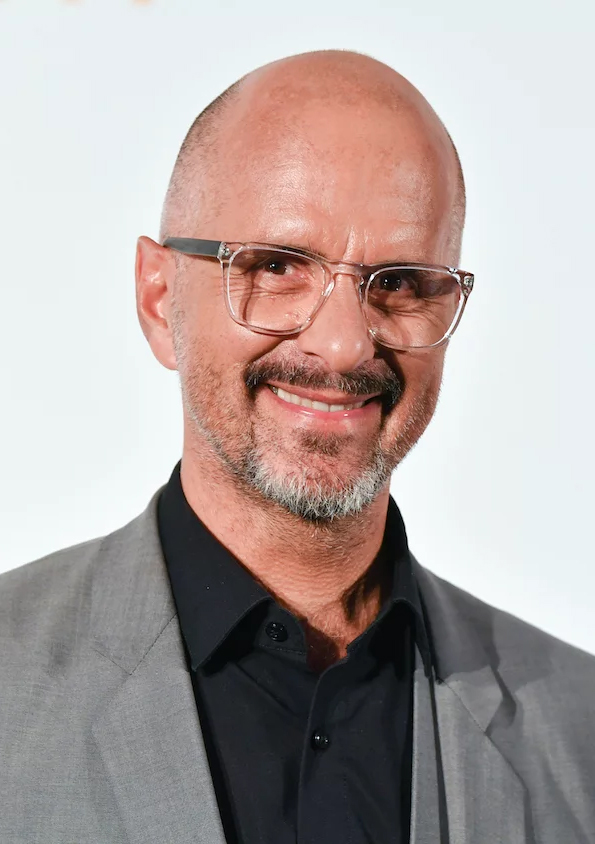
\includegraphics[width=0.8\textwidth]{Fotos/ChristophMariaHerbst.jpg}
    \label{fig:ChristophMariaHerbst} % Label für Querverweise
\end{figure}

\addchap{Warum es dieses Buch gibt}
\addcontentsline{toc}{chapter}{Warum es dieses Buch gibt}

\textit{„Wie kommst Du damit klar?“}, fragte mich die Frau ganz direkt. Wir hatten bereits eine Zeit lang über dies und das geplaudert. Gemeinsam mit der pädagogischen Leiterin der Einrichtung saßen wir im Leseraum des Kinder- und Jugendhospizes Olpe und ich überlegte, wie ich ihre Frage beantworten wollte. Es ging um die Krankheit, an der ich leide: eine fortschreitende Form von Muskelschwund. Die Antwort, die ich ihr dann gab, klingt vielleicht banal: \textit{„Man wächst einfach hinein.“} Und genauso ist es.

Das war 2020 während eines Aufenthalts im Balthasar. Ich war gerade angekommen. Meine Eltern hatten die Koffer ausgeräumt, meine Klamotten in den Schränken verstaut, Laptop und Playstation angeschlossen und sich nach der üblichen Abschiedszeremonie auf den Heimweg gemacht. Anja Schulte, die damalige pädagogische Leiterin, kam in mein Zimmer und fragte mich, ob ich Zeit und Lust auf ein Gespräch hätte. Die Mutter eines sechsjährigen Jungen, der ebenfalls mit Duchenne Muskeldystrophie auf die Welt gekommen war, wollte die Gelegenheit nutzen und sich mit jemandem austauschen, der an der gleichen Krankheit litt wie ihr Sohn. Jemand, der sozusagen aus erster Hand berichten und ihr Tipps geben konnte.
Natürlich hatte ich Zeit. Und Lust.

So trafen wir uns noch am gleichen Nachmittag. Die Frau war ziemlich taff; sie erinnerte mich an meine Mutter. In ihrem Sohn, der mir zuvor schon im Aufenthaltsbereich aufgefallen war, sah ich mich selbst vor über 20 Jahren. Ich beantwortete ihre Fragen so gut ich konnte, beispielsweise welche medizinischen Eingriffe ich hinter mir habe, warum ich mich für die eine oder andere Operation entschieden habe, welche Hilfsmittel ich in der Vergangenheit in Anspruch genommen habe und welche ich zurzeit nutze, aber auch wie meine Erfahrungen mit den Krankenkassen sind und welche Therapien ich mache.

Die Zeit flog nur so dahin. Obwohl das Gespräch über zwei Stunden dauerte, kam es mir vor wie zehn Minuten. Ich hoffe sehr, dass ich der Frau habe helfen können, indem ich ihr von meinem Leben mit der Krankheit erzählte und von meinen Erfahrungen, in der Kindheit, der Jugend, bis zum heutigen Tag. Vielleicht konnte ich ihr auch vor Augen führen, dass man als Mittzwanziger mit Duchenne durchaus zuversichtlich und lebensbejahend sein kann und nicht zurückgezogen und in sich gekehrt sein muss – was wohl viele denken – und dass die Krankheit das Leben der Betroffenen und ihrer Familien zwar in vielen Bereichen beherrscht, aber eben nicht komplett.

Für mich war das Gespräch mit dieser Mutter eine Bereicherung. Hört sich jetzt etwas pathetisch an, aber ich spürte das Geschenk des ehrlichen Interesses, des aufmerksamen Zuhörens und des Dankes. Das inspirierte mich. Als die Einrichtungsleitung des Balthasars einige Wochen später auf mich zukam und mich fragte, ob ich mir vorstellen könne, ein Buch über mich und meine Krankheit zu schreiben, musste ich nur kurz überlegen. Früher hätte ich mir ein solches Projekt nicht zugetraut. Jetzt aber gehe ich dieses Wagnis ein, auch wenn es mich einiges an Überwindung kostet, immerhin gebe ich viel von mir Preis.

\noindent Aber alles der Reihe nach …

\begin{figure}[H]
    \raggedright
    \includegraphics[width=0.45\textwidth]{Fotos/Marius.jpg}
\end{figure}
\noindent\small\textit{Grevenbroich, September 2024}

%\clearpage
%\tableofcontents % Hier wird das Inhaltsverzeichnis eingefügt
%\clearpage

\mainmatter

\clearpairofpagestyles % Setzt alle Kopf-/Fußzeilen zurück
\rehead{\leftmark}     % Gerade Seiten: Kapitelüberschrift rechts
\lehead{\thepage}      % Gerade Seiten: Seitenzahl links
\rohead{\thepage}      % Ungerade Seiten: Seitenzahl rechts
\lohead{\leftmark}     % Ungerade Seiten: Kapitelüberschrift links

\pagestyle{scrheadings}

\addchap{Die ersten Jahre}
\thispagestyle{scrheadings} % Wichtig, sonst erscheint die Kopfzeile nicht auf der ersten Seiet des Kapitels
\addcontentsline{toc}{chapter}{Die ersten Jahre}

\leavevmode
\vspace*{0.5\baselineskip}
{\noindent\fontsize{18}{24}\selectfont\textcolor{myblue}{Ich, Wunschkind}\par}
{\noindent\fontsize{14}{20}\selectfont\scshape\textcolor{myblue}{Eigentlich lief alles bestens}\ldots\par}
\vspace*{0.5\baselineskip}
\normalsize

\noindent Was ist deine früheste Kindheitserinnerung? Und wie alt warst du da? Man sagt, dass die Grenze für früheste Erinnerungen zwischen drei und vier Jahren liegt. Um euch also über meine ersten Lebensjahre berichten zu können, musste ich meine Eltern, Elke und Peter, interviewen. Wir drei haben ein sehr gutes und inniges Verhältnis zueinander. Und meine Fragen über diese Phase meines Lebens haben sie gerne und ausführlich beantwortet. Apropos: falls ihr euch fragt – ich bin Marius, 29 Jahre alt.

Offenbar war ich ein lang ersehntes Wunschkind. Meine Eltern hatten sich jedenfalls riesig gefreut, als feststand, dass meine Mutter mit mir schwanger war. So wie sich alle Eltern freuen, die sich ein Kind wünschen. Die ersten drei Monate einer Schwangerschaft sind ja die kritischsten. Wie man nachlesen kann, übernimmt die Plazenta etwa ab der 12. Schwangerschaftswoche die vollständige Versorgung des Fötus. Danach sinkt das Risiko einer Fehlgeburt drastisch. Dementsprechend vorsichtig war meine Mutter während dieser Zeit und gab besonders gut auf uns beide acht. Wir kamen gut durch diese Phase und auch die übrigen 26 Wochen der Schwangerschaft.

Auf die Welt kam ich schließlich im Mai 1995 im Kreißsaal des Elisabeth-Kran\-ken\-hau\-ses in Grevenbroich. Auf den Tag genau, so wie es die Geburtsberechnung vorausgesagt hatte. Ich kam mit dem Kopf voran und mein jetziges, dunkelblondes Haar war bei der Geburt und auch einige Wochen danach noch schwarz. Getauft wurde ich auf den Namen Marius. Im Wettstreit der Vornamen hatten die Konkurrenten Oskar und Luis das Nachsehen. Zum Glück. Denn ist es nicht so, hat man erst einmal einen Vornamen, kann man sich einen anderen irgendwie nicht mehr vorstellen?

Apropos Namen: Den Namen Grevenbroich habt ihr vermutlich schon einmal gehört. Grevenbroich ist diese kleine Stadt, gelegen auf der linken Rheinseite im Dreieck Köln-Düsseldorf-Mönchengladbach, die bei Umweltschützern wegen der Braunkohleförderung im riesigen Tagebau Garzweiler zu zweifelhaftem Ruhm gekommen ist. 2030 soll damit Schluss sein. Grevenbroich wurde aber auch durch die von Hape Kerkeling verkörperte Kunstfigur Horst Schlämmer, seines Zeichens nuschelnder Chefredakteur des fiktiven Grevenbroicher Tagblattes, deutschlandweit bekannt.

\begin{figure}[ht]
    \centering
    \includegraphics[width=\textwidth]{Fotos/Grevenbroich_in_Google_Earth.png}
    \caption{Grevenbroich hat etwa 67.000 Einwohner und liegt im Braunkohlerevier westlich von Köln. Die ockerfarbenen Flecken auf der Karte sind Tagebaue, riesige, hunderte Meter tiefe Löcher, in denen gigantische Schaufelradbagger Braunkohle fördern.}
    \label{fig:grevenbroich}
\end{figure}

In diesem Städtchen also, genauer gesagt in seinem südlichsten Stadtteil Neurath, lebe ich seit meiner Geburt gemeinsam mit meinen Eltern, Kater Smokie sowie dem langhaarigen holländischen Hütehund Gonzalo. Ich war das erste Kind meiner Eltern und sollte auch das einzige bleiben. Nach Neurath kamen meine Eltern im November 1990, etwa fünf Jahre vor meiner Geburt. Beide sind gebürtige Grevenbroicher. Sie lebten bereits seit drei Jahren zusammen und hatten sich wegen einer aus ihrer Sicht unverschämten Mieterhöhung auf die Suche nach einem eigenen Haus gemacht. In Neurath wurden sie schließlich fündig.

Das Haus, in dem ich die ersten acht Jahre meines Lebens verbracht habe, ist eine zweieinhalbgeschossige Doppelhaushälfte aus den 50er Jahren. Keine Schönheit, aber einigermaßen gut in Schuss. Zum Zeitpunkt meiner Geburt gehörten auch die Bernhardiner-Dame Bianca und die beiden Kater Max und Felix mit zur Familie. Bianca litt leider an einem bösartigen Knochentumor am vorderen Lauf, der sich nicht operieren ließ. Mit vier Jahren haben meine Eltern sie auf Anraten des Tierarztes einschläfern lassen. Eine Erinnerung an sie habe ich nicht. Allerdings gibt es ein Foto, das sie neben meinem Kinderwagen sitzend zeigt. Mit den beiden Katern habe ich noch einige Jahre zusammen verbracht. Hunde und Katzen gehören von Anfang an zu meinem Leben. Sie haben mir immer viel Freude bereitet und mich oft zum Lachen gebracht. Ich bin fest davon überzeugt, dass Haustiere das Leben ihrer Besitzer positiv beeinflussen.

\setlength{\fboxsep}{0pt}    % Kein Abstand zwischen Rahmen und Bild
\setlength{\fboxrule}{0.2pt} % Rahmenstärke auf 0.2 pt setzen
\begin{figure}[ht]
    \centering
    \fcolorbox{rahmenlinie}{white}{\includegraphics[width=1\textwidth]{Fotos/Zeltgemeinschaft.jpg}}
    \caption{Der Schapendoes-Rüde Rudi hat mich viele Jahre begleitet. Aufgenommen wurde das Foto an einem Strand in der niederländischen Provinz Zeeland. Ein Leben ohne Haustiere ist für mich unvorstellbar.}
    \label{fig:zeltgemeinschaft}
\end{figure}

Zurück zum Haus. Wenn meine Eltern gewusst hätten, dass ihr Kind früher oder später auf einen Rollstuhl angewiesen wäre, hätten sie sich nicht für dieses Haus entschieden. Sie haben es aber weder gewusst noch haben sie es geahnt. Wie auch? Nichts deutete in den ersten zwei Jahren meines Lebens darauf hin. In Sachen Barrierefreiheit war das Haus eine Katastrophe. Mein Kinderzimmer, das mein Vater während der Schwangerschaft hergerichtet hatte und das von meinen Eltern liebevoll eingerichtet worden war, lag direkt unter dem Dach, zwei ziemlich steile Treppen vom Erdgeschoss entfernt. Ich kann mich noch daran erinnern, dass ich mich diese Treppen mühsam hinaufgeschleppt habe, beide Hände das Geländer fest umklammernd. Meine Schritte beim Treppensteigen waren dabei nicht alternierend. Das bedeutet, dass ich den ersten Fuß auf eine Stufe gesetzt habe und anschließend den zweiten Fuß auf dieselbe und nicht etwa auf die nächsthöhere Stufe. Ein typisches Anzeichen für eine Muskelschwäche.

Der Zugang zum Haus stellte ebenfalls eine Hürde dar, denn selbst das Erdgeschoss befand sich nicht auf Straßenniveau. Wie bei vielen Häusern, die in den 50er und 60er Jahren gebaut worden waren, musste man erst ein paar Stufen erklimmen, bevor man vor der Haustür stand. Und auch in den Garten kam man nur über eine Treppe. Von der reinen Quadratmeterzahl her bot das Haus locker Platz für bis zu vier Personen. Aber die Wohnfläche verteilte sich auf drei Etagen. Rollstuhl, Treppenlift, Aufzug? Undenkbar.

Die ersten zwei Jahre meines Lebens waren unspektakulär. Ich lernte nach und nach alle Familienmitglieder kennen, wurde auf Familienfeiern herumgereicht, aß und trank gut und wuchs zu einem Wonneproppen heran, der sich in nichts von anderen zweijährigen Wonneproppen unterschied.
Zumindest nicht auf den ersten Blick.

\section{Da stimmt was nicht}
Rückblickend betrachtet, so meine Mutter, gab es sehr wohl Anzeichen. Allerdings subtile, die man als Argloser nicht unbedingt zu deuten vermochte. Ich krabbelte beispielsweise nicht, so wie es viele (wenn auch nicht alle) Kleinkinder tun, bevor sie laufen lernen. Und ich war seit meinem ersten Lebensjahr heiser. In einer Situation fiel meiner Mutter auch auf, dass es mich Kraft kostete, wenn ich auf dem Bauch lag und den Kopf anheben wollte. Aber da ich schließlich mit 16 Monaten das Laufen erlernte, lösten sich diese ersten Bedenken, dass mit mir körperlich vielleicht etwas nicht stimmte, erstmal in Luft auf.

Meine Mutter hatte mich ein halbes Jahr nach meiner Geburt bereits in einem Kindergarten angemeldet, den ich mit dreieinhalb Jahren dann auch besuchte. Ein Jahr zuvor bin ich bereits regelmäßig in eine Spielgruppe gegangen (in der ich meinen ältesten Freund Marvin kennengelernt habe, zu dem ich heute noch Kontakt halte, auch wenn er zwischenzeitlich nach Berlin gezogen ist).

Gegen Ende meiner Zeit in dieser Spielgruppe fiel einer der beiden Pädagoginnen auf, dass ich offensichtlich Plattfüße und einen Watschelgang hatte. Beides sind Anzeichen für Duchenne Muskeldystrophie. Diese Art zu gehen, entsteht aufgrund der Schwäche der Hüft- und Gesäßmuskulatur. Um die Schwäche in der Hüfte auszugleichen und eine möglichst stabile Körperhaltung einzunehmen, machen Duchenne-Jungen ein Hohlkreuz und wölben den Bauch nach vorne. Wenn man in dieser Haltung barfuß geht, Plattfüße hat, weil das Fußgewölbe nicht richtig ausgebildet ist, und man den Fuß auch nicht abrollen kann, dann hat dieser Gang etwas von Watscheln. Duchenne Muskeldystrophie erkläre ich euch auf Seite 119 noch genauer.

\section{„Ach was! Das kommt noch!“ Denkste!}

Auch wenn man diese Fehlhaltung anfangs vielleicht noch mit einem „Ach was! Nicht alle Kinder sind gleich flink und beweglich. Das kommt schon noch!“ abtut, so schaut man nach einem solchen Fingerzeig vielleicht doch etwas genauer hin. Während man anfangs noch darüber hinwegsah, so waren die eigentümliche Körperhaltung mit vorgewölbtem Bauch und der tapsige Gang spätestens von da an unübersehbar geworden. Aber sie waren längst noch nicht beunruhigend. Wofür gibt es schließlich Physiotherapeut:innen? Man riet uns denn auch, eine solche aufzusuchen, um den Plattfuß und die vermeintlich daraus resultierende Fehlhaltung (wie meine Eltern fälschlicherweise glaubten) frühzeitig zu behandeln.
              
\section{Gowers-Manöver und die Schwierigkeit aufzustehen}

Alles gut? Leider nicht. Denn es wurde immer offensichtlicher, dass ich meinen Altersgenossen körperlich immer mehr hinterherhinkte. Vom Boden aufzustehen, fiel mir besonders schwer. Ich musste mich immer erst hinknien und dann mit dem Arm am Oberschenkel hochdrücken, um in den aufrechten Stand zu kommen. Diese Art sich aufzurichten, wird als Gowers-Manöver bezeichnet. Es ist typisch für Duchenne Muskeldystrophie.

\section{Ich kann nicht so schnell}

Eine Situation hat sich bei meiner Mutter besonders eingeprägt. Wir hatten mit der Spielgruppe eine Waldwanderung unternommen und die Kinder trafen nach und nach am vereinbarten Ort ein, um von ihren Eltern in Empfang genommen zu werden. Die letzten, die dort viele Minuten nach den anderen ankamen, waren meine Spielgefährtin Janine und ich, gefolgt von einer erwachsenen Begleiterin. Ich konnte einfach nicht so schnell. Gehen kostete mich Kraft und ich stolperte auch immer häufiger, weil ich meine Füße beim Gehen nicht mehr ausreichend anheben konnte.

Als sich meine Eltern auf Anraten der Pädagogin dieser Spielgruppe dazu entschlossen hatten, mit mir einen Physiotherapeuten aufzusuchen, war es aus ihrer Sicht eigentlich nur eine Frage der Zeit, bis meine Beeinträchtigungen auskuriert wären und ich zu meinen Altersgenossen körperlich wieder aufschließen würde.

\section{Physiotherapie half auch nicht}

Nach einer Reihe von Physiotherapie-Sitzungen stellte sich der erhoffte Erfolg jedoch nicht ein. Die erste Praxis behandelte nach dem Ansatz von Bobath. Diese Methode wird bei Erwachsenen und Kindern mit neurologischen Erkrankungen angewendet, zum Beispiel bei Menschen, die nach einem Schlaganfall halbseitig gelähmt sind. Das Konzept beruht auf der Annahme, dass sich das Gehirn umorganisieren lässt, dass gesunde Hirnregionen Aufgaben neu lernen und übernehmen können, die zuvor von erkrankten Hirnregionen ausgeführt worden waren. Duchenne ist jedoch keine neurologische Erkrankung, von daher änderte die Behandlung natürlich auch nichts an meinem Zustand.

Man riet meinen Eltern, es mit einem anderen physiotherapeutischen Ansatz zu versuchen. Bei der Vojta-Therapie sollen Bewegungsstörungen durch eine Stimulation, nämlich das Auslösen von Reflexen, also auf einen bestimmten Reiz hin stets gleich ablaufende Reaktionen, die nicht bewusst gesteuert werden können, behoben werden. Für Vojta gilt das gleiche wie für Bobath: Duchenne ist eine muskuläre Erkrankung, die körperlichen Beeinträchtigungen sind Folge eines Absterbens von Muskelzellen – Reflextherapien beheben solche muskulären Defekte nicht.

Die dritte Physiotherapeutin (diese Praxis betreut mich übrigens bis heute) riet uns schließlich, mein Problem besser einmal medizinisch begutachten zu lassen. Der Kinderarzt, der mich von Geburt an behandelte und meine Eltern beraten hatte, war zwischenzeitlich in den Ruhestand gegangen. So vereinbarten sie einen Termin bei einem Kinderarzt, der seine Praxis in Grevenbroich gerade neu eröffnet hatte. Ihm erzählten sie also im Dezember 1998 meine Geschichte und dass keine der Physiotherapien auch nur eine leichte Besserung bewirkt hatte.

\section{Das Ende der unbeschwerten Jahre}

Der Arzt entnahm mir eine Blutprobe und ließ sie im Labor untersuchen. Wir hatten vor, das Weihnachtsfest und den Jahreswechsel gemeinsam mit meinen Großeltern im Erzgebirge zu verbringen. Meine Eltern erwähnten dies dem Arzt gegenüber wohl mehr oder weniger beiläufig. Denn obwohl das Ergebnis der Blutuntersuchung bereits vor unserer Abreise feststand, teilte man es meinen Eltern sozusagen aus Rücksicht auf ein paar unbeschwerte Feiertage erst nach unserer Rückkehr am 11. Januar 1999 mit. Der Creatinkinase Wert (CK) in meinem Blut war deutlich erhöht. Das Enzym Creatinkinase ist für den Energiestoffwechsel der Muskelzellen wichtig. Sind die Zellen geschädigt, etwa durch einen Herzinfarkt, Sturz oder wie in meinem Fall durch das Fehlen des Proteins Dystrophin (daher auch der Name Muskeldystrophie), findet sich vermehrt Creatinkinase im Blut. Der Normalwert liegt bei einem Gesunden in meinem Alter bei weniger als 150 Einheiten pro Liter Plasma. Bei mir waren es 7.000.
Die unbeschwerten Jahre waren damit vorbei.

Was die Diagnose Duchenne Muskeldystrophie bedeutete, war mir natürlich nicht klar. Aber von dem Moment der Diagnose an änderte sich mein Leben und das meiner Eltern schlagartig und dauerhaft. Ihnen wurde der Boden unter den Füßen weggezogen. Unser altes Leben, das noch wenige Wochen zuvor unbekümmert und glücklich war, rückte mit einem Schlag unwiederbringlich in weite Ferne und wurde zu etwas langsam Verblassendem, an das sie sehnsüchtig zurückdachten. Es sollten zwei Jahre vergehen, bis der Horror zumindest teilweise verarbeitet worden war und das Glück nach und nach in unsere Familie zurückkehrte.

\section{Was tun? Aktion Benni \& Co.}

Was tun Eltern, die soeben erfahren haben, dass ihr nicht einmal vier Jahre alter Sohn an einer fortschreitenden und tödlich verlaufenden Muskelkrankheit litt? Meine beschäftigten sich von dem Moment an intensiver mit dieser Krankheit. Beim Stöbern im Internet (Google war damals übrigens gerade mal ein Jahr alt) stießen sie auf die im Westerwald beheimatete Elterninitiative Aktion Benni \& Co. Diese war 1996, also ein Jahr nach meiner Geburt, von den Eltern des ebenfalls an Duchenne Muskeldystrophie erkrankten Benni gegründet worden.

Ziel der Initiative war es, Geld zu sammeln, um damit die Forschung in Bezug auf eine Heilung der Duchenne Muskeldystrophie zu intensivieren. Aktion Benni \& Co. ist mittlerweile in dem eingetragenen Verein Duchenne Deutschland e.~V. aufgegangen.

\begin{mdframed}[
    linewidth=0.3pt,         % Dünne Linie
    linecolor=rahmenlinie,   % Deine definierte Rahmenfarbe
    leftmargin=0, rightmargin=0,
    innertopmargin=8pt, innerbottommargin=8pt,
    innerleftmargin=12pt, innerrightmargin=12pt,
    backgroundcolor=white
]
\small\sffamily
\setlength{\parindent}{0pt} % Kein Erstzeileneinzug

\vspace{0.2\baselineskip}
\textbf{Duchenne Deutschland e.\,V. und Deutsche Duchenne Stiftung}

Duchenne Deutschland e.~V. ist eine Initiative von Eltern, deren Kinder Duchenne Muskeldystrophie (DMD) haben. Mit seiner Arbeit, die größtenteils von ehrenamtlichen Helfern geleistet wird, unterstützt der Selbsthilfeverein Betroffene und ihre Familien durch Beratung und Information in allen Lebensphasen.

\vspace{0.8\baselineskip}

Zweck des Vereins ist auch die Förderung von Wissenschaft und Forschung. Mit Spendengeldern unterstützt er – in Absprache mit einem wissenschaftlichen Beirat – die DMD-Forschung sowie Studien und fördert die Kommunikation und die Zusammenarbeit der weltweit mit DMD befassten Wissenschaftler. Der Verein informiert Patienten und ihre Familien über aktuelle und geplante Forschungsprojekte und richtet Veranstaltungen wie das jährliche Duchenne-Symposium oder regelmäßige Web-Konferenzen aus.

\vspace{0.8\baselineskip}

Die Deutsche Duchenne Stiftung (\url{https://www.duchenne-deutschland.de}) wurde 2010 als selbständige Stiftung gegründet, um die Arbeit für die Duchenne-Gemeinschaft dauerhaft zu sichern, die Forschung zur Entwicklung von Therapien zu forcieren und die Lebenssituation der Betroffenen zu verbessern. Aufklärung der Öffentlichkeit sowie die Umsetzung sozialer und psychologischer Projekte für DMD-Familien sind weitere Bestandteile der Stiftungsarbeit.\\

\vspace{0.8\baselineskip}
\textbf{Deutsche Duchenne Stiftung – Duchenne Deutschland e.~V.}

Huestraße 20, 44787 Bochum\\
Telefon: +49 234 925 696 70\\
Fax: +49 234 925 696 72\\
E-Mail: info@duchenne-deutschland.de\\
Webseite: \url{https://www.duchenne-deutschland.de}

\vspace{0.8\baselineskip}
\textbf{Spendenkonten}

Duchenne Deutschland e.~V.\\
Sparkasse Bochum\\
IBAN: DE67 4305 0001 0000 4277 24\\
BIC: WELADED1BOC\\
Deutsche Duchenne Stiftung\\
Volksbank Ruhr Mitte\\
IBAN: DE44 4226 0001 0603 1297 00

\end{mdframed}

\vspace{0.8\baselineskip}

\noindent Auch wenn Duchenne Muskeldystrophie die häufigste muskuläre Erbkrankheit im Kindesalter ist und statistisch etwa jeder 3.500ste Junge an ihr erkrankt, ist ihre Häufigkeit dennoch verschwindend gering im Vergleich zu Erkrankungen des Herz-Kreislauf-Systems, Krebs oder Diabetes. Alleine im Jahr 2020 gab es über eine halbe Million neudiagnostizierte Krebserkrankungen.

Für Pharmaunternehmen ist der Markt der Volkskrankheiten deutlich lukrativer als der eher übersichtliche Markt der neuromuskulären Erkrankungen wie Duchenne. Mit der kostspieligen Entwicklung von Medikamenten und Therapien lässt sich in diesem Segment schlicht kein Geld verdienen, und als Folge davon kommt auch die Forschung zu kurz. Und wenn an Duchenne Muskeldystrophie nicht geforscht wird, dann wird es weder mittelfristig noch langfristig Hoffnung auf Heilung geben. Das möchten in Deutschland Vereine wie seinerzeit Aktion Benni \& Co., heute Duchenne Deutschland e.~V., oder in den USA Parent Project DMD ändern: sie machen die Öffentlichkeit auf die Krankheit aufmerksam und sammeln Spendengelder zur Unterstützung der Forschung mit Blick auf eine Heilung der Erkrankung.

Meine Eltern traten also dem Verein Aktion Benni \& Co. bei. Sie machten in und um Grevenbroich auf die Krankheit Duchenne Muskeldystrophie aufmerksam und sammelten fleißig Spendengelder. Damit begann eine Zeit mit vielen Benefizveranstaltungen, Fototerminen und Scheckübergaben. Wir tauchten in etlichen Zeitungsartikeln auf und machten mit unserer Geschichte das Thema Duchenne Muskeldystrophie einer größeren Öffentlichkeit bekannt.

Dies hatte dann auch den gewünschten Schneeballeffekt zur Folge: Denn nicht nur unsere Familien waren eifrig dabei, Spendengelder zu sammeln, auch Freunde und Bekannte legten sich mächtig ins Zeug, um unser Anliegen publik zu machen. Sie sprachen ihre Freunde, Bekannten und auch Firmen an und sorgten schließlich dafür, dass innerhalb von zwei Jahren mehr als 100.000 DM aus unserem Postleitzahlbezirk auf das Spendenkonto von Aktion Benni \& Co. eingezahlt wurden!

Meine Eltern erzählten mir, dass ihnen die vielen Aktivitäten rund um Aktion Benni \& Co. zwar nicht dabei halfen, die Realität um sie herum komplett auszublenden und den Horror ganz zu vergessen, man sah mir die Krankheit ja an, für deren Bekämpfung sie Spendengelder sammelten. Aber es lenkte sie zumindest ab. Sie hatten eine Aufgabe, auf die sie ihre Gedanken fokussieren konnten. Und mit jeder gespendeten (damals noch) DM, so hofften sie, würde auch die Heilung ihres Sohnes ein Stück näher rücken. Die beiden engagierten sich etwa zwei Jahre für Aktion Benni \& Co. und beschlossen dann, sich wieder mehr auf die Familie, auf uns drei zu konzentrieren. Dafür gab es einen guten Grund: Wir planten den Bau eines behindertengerechten Hauses.

\section{Wir bauen ein Haus}

Rückblickend war 2001 ein wirklich besonderes Jahr, weil in jenen 12 Monaten so viel passiert ist. Zum einen war im Spätsommer die Zeit des sorglosen Spielens, Bastelns und Singens im Kindergarten „Villa Kunterbunt“ vorbei. Ich war im Mai sechs geworden und kam in die Schule, so wie viele andere Sechsjährige auch. Ich kann mich nicht mehr daran erinnern, ob ich mich auf die Schule gefreut habe oder aber der Kindergartenzeit hinterhertrauerte. Wahrscheinlich tat ich beides. Von meiner Schulzeit werde ich später noch berichten. Zunächst möchte ich euch von dem bis dahin größten Projekt meiner Eltern erzählen, dem Bau eines behindertengerechten Hauses.

Ich kann mir vorstellen, dass es eine ganz besondere Herausforderung ist, ein Haus zu planen und zu bauen. Man bindet sich nicht nur für viele Jahre an eine Bank, sondern man entscheidet auch, wo man in Zukunft leben möchte und wo sich das Leben der Familie abspielen wird. Meine Eltern entschieden sich, in Neurath zu bauen.

Die Doppelhaushälfte in Neurath, die die beiden 1990 gekauft hatten und in der sie insgesamt 13 Jahre lang lebten, war acht Jahre lang mein Zuhause. Das Haus war Mitte der 50er Jahre gebaut worden und architektonisch nicht unbedingt ein Schmuckstück. Aber das können die wenigsten Häuser aus dieser Zeit von sich behaupten. Es verfügte über einen hübschen, kleinen Garten, in dem ein alter Kirschbaum stand, an dessen dickem Ast eine Schaukel hing, die mein Vater aus einem abgefahrenen Autoreifen und einem Seil gebaut hatte. Am Ende des Gartens befand sich ein ziemlich großes Gartenhaus, das sowohl auf unserem als auch auf dem Grundstück unserer Nachbarn stand, und das meine Eltern gemeinsam mit den Nachbarn schon vor meiner Geburt gebaut hatten. Unser Haus lag ziemlich zentral, etwas abseits der Dorfmitte Neuraths, nicht weit entfernt vom Kindergarten und direkt gegenüber der Grundschule.

\section{Unser erstes Zuhause, das Gegenteil von barrierefrei}

So sehr wir drei unser Zuhause auch liebten, hatte es doch einen gravierenden Nachteil: Es war das genaue Gegenteil eines behindertengerechten und barrierefreien Hauses. In der Zeit, als es gebaut wurde, war der Begriff „Barrierefreiheit“ noch nicht im Duden aufgeführt, und ob man mit dem Rollstuhl in ein öffentliches oder privates Gebäude kam, interessierte vor 70 Jahren niemanden. Zum Teil auch heute noch nicht.

Natürlich hatte ich als kleiner Junge überhaupt keine Ahnung, was Barrierefreiheit bedeutete und ebenso wenig wusste ich, dass die beengten Verhältnisse in unserem Haus für eine:n Rollstuhlfahrer:in ein echtes Problem darstellten. Ich war klein, hatte ganz andere Dinge im Kopf und konnte ja schließlich noch laufen. Allerdings ahnte ich damals schon, dass mit dem Haus irgendetwas nicht stimmt. Ich konnte zwar trotz der allmählich schwindenden Muskulatur in meinen Beinen noch im Erdgeschoss umherlaufen (und fiel dabei das eine oder andere Mal auch hin), ich schaffte es jedoch nicht, aus eigener Kraft in mein Kinderzimmer im zweiten Stock zu gelangen. Zwar kämpfte ich mich in ganz jungen Jahren noch alleine die Stufen hoch, später jedoch war es ganz selbstverständlich, dass meine Eltern mich die beiden steilen Treppen in mein Zimmer hochtrugen. Heruntersteigen konnte ich die Treppen anfangs noch alleine. Allerdings auch das nie, ohne dass meine Eltern danebenstanden, um auffangen zu können, falls ich stolperte. Damit musste man bei mir immer rechnen.

\section{Meine Angst vor Rollstühlen}

Mit der Diagnose Duchenne Muskeldystrophie stand unweigerlich fest, dass ich früher oder später einen Elektro-Rollstuhl brauchen würde, um mich eigenständig fortbewegen zu können. Ein Thema, das meine Eltern anfangs komplett ausgeblendet hatten. Mich im Rollstuhl sitzen zu sehen, war etwas, mit dem sie sich in den ersten beiden Jahren nach der Diagnose nicht befassen wollten oder konnten. Der Rollstuhl war nicht nur ein Hilfsmittel zur Fortbewegung und zum Erhalt der Selbstständigkeit. Er war auch ein Symbol. Ein Symbol dafür, dass mit dem Verlust meiner Gehfähigkeit für alle sichtbar das nächste Stadium der Krankheit begonnen hatte. Mit dem Rollstuhl würde eine neue Phase in meinem Leben anbrechen, die ich von da an im Sitzen und auf Rädern meistern musste, ob ich wollte oder nicht. Das zu akzeptieren, fiel anfangs nicht nur meinen Eltern schwer, sondern mir auch. Denn ich hatte Angst vor Rollstühlen.

Klingt komisch, aber war tatsächlich so. Es gibt eine Situation, die mir heute fast wie eine sich selbst erfüllende Prophezeiung vorkommt (ich bin allerdings nicht abergläubisch). Meine Eltern waren immer schon bekennende Camper. Eigentlich sind sie es immer noch, aber leider machen die Umstände das Zelten so gut wie unmöglich, der logistische Aufwand ist einfach riesig. Früher, als ich noch gehen konnte, aber auch noch, als ich schon im e-fix saß, haben wir viele unserer Urlaube und verlängerten Wochenenden an der holländischen Küste auf einem Campingplatz in der Nähe vor Domburg verbracht. Dazu auf Seite 67 mehr.

Es war vielleicht im Sommer 1999 oder 2000, als ich auf diesem Campingplatz zum ersten Mal einen Jungen in einem Elektro-Rollstuhl sah. Der Rollstuhl erschien mir riesig und er machte mir Angst. Anders als ich und alle anderen Menschen, die ich kannte, ging der Junge nicht auf zwei Beinen, sondern er fuhr mit diesem Ding umher, das zu allem Schrecken dieses seltsam summende Geräusch von sich gab. Ich konnte kaum hinschauen und ging dem Jungen falls möglich aus dem Weg. Dass ich keine zwei Jahre später selbst auf einen Rollstuhl angewiesen sein würde (zumindest zeitweise), ahnte ich natürlich nicht. Es würde zur Ironie des Schicksals passen, wäre der Junge so wie ich an Duchenne Muskeldystrophie erkrankt und ich sozusagen einen Blick meiner eigenen Zukunft erhascht hätte. So viel zur Angst vor Rollstühlen. Klar, die Angst war spätestens verschwunden, als ich selbst in einem saß.

\section{Treppen und Rollstuhl? Unmöglich.}

Doch zurück zum Haus. Auch wenn meine Eltern das Thema Rollstuhl emotional auf Distanz hielten, so war ihnen doch schon mit der Diagnose klar, dass das Haus ein Problem darstellte, mit dem man sich früher oder später befassen musste. Spätestens dann, wenn sich abzeichnete, dass ich einen Rollstuhl bräuchte.
Doch welche Optionen gab es? Die auf den ersten Blick naheliegendste war ein Umbau des Hauses. Doch das war nicht so einfach, um nicht zu sagen unmöglich. Das Erdgeschoss hatte eine Fläche von etwa 50 Quadratmetern und bot Platz für ein Wohnzimmer, ein Gäste-WC und die Küche. Es lag gut einen Meter über Straßenniveau und war nur über eine Außentreppe erreichbar. Diesen Niveauunterschied hätte man mit einer langen Rampe überwinden können. Doch mit welchem Ergebnis? Ich wäre mit dem Rolli zwar ins Haus gekommen, aber spätestens dort wäre mit der Barrierefreiheit Schluss gewesen.

Wie gesagt, es war alles ziemlich beengt und wichtige Räume wie Bad und Kinderzimmer lagen im ersten bzw. zweiten Obergeschoss. Wie sollte ich im Rollstuhl dorthin kommen? Dafür hätte man einen Außenaufzug benötigt. Auch den hatten meine Eltern in Erwägung gezogen. Allerdings gab es keine geeignete Wand, an die man den Aufzug von außen hätte montieren und wo man die Fassade hätte durchbrechen können, um ins Hausinnere zu gelangen. Selbst wenn, so wäre ein Aufzug bautechnisch nur bis ins erste Obergeschoss möglich gewesen. Bis unter das Dach, wo mein Kinderzimmer lag, hätte man ihn nicht bauen können. Es wurde meinen Eltern recht schnell klar, dass Aufwand und Nutzen eines solchen Vorhabens in keinem vernünftigen Verhältnis standen. Ein Außenaufzug hätte sehr aufwändige und teure Umbaumaßnahmen im Hausinneren erforderlich gemacht und wäre doch immer ein fauler Kompromiss geblieben, über den man sich später ärgern würde.

\section{Entscheidung Neubau}

Am Ende entschieden sie sich dazu, neu zu bauen. Und zwar in Neurath. Für meine Eltern war es damals wichtig, dass wir dortblieben. Eine Entscheidung, die sie heute zwar nicht unbedingt bereuen, die sie aber unter Umständen nicht mehr so treffen würden. Einer der wichtigsten Gründe, nicht aus Neurath wegzuziehen, war das soziale Umfeld, in dem ich groß geworden war. Ich besuchte den dortigen Kindergarten und lernte in den drei Jahren viele Kinder kennen, mit denen ich auch nachmittags oft spielte. Außerdem wechselte ich ja auf die Grundschule in Neurath, wo ich viele meiner Spielgefährt:innen aus der Kindergartenzeit wieder treffen würde.

Im Kreise all der Kinder, die mich und meine Krankheit schon aus der Kindergartenzeit kannten, wäre ich gut aufgehoben, so dachten meine Eltern damals, als diese wichtige Entscheidung anstand. Der Tatsache, dass sich die Wege nach der Grundschulzeit in der Regel trennen, hatten sie dabei weniger Beachtung geschenkt. Ehemalige Spielgefährt:innen oder Klassenkamerad:innen laufen mir in Neurath jedenfalls so gut wie nie über den Weg. Vielleicht wäre ein Umzug zum Beispiel nach Köln besser gewesen, weil in einer großen Stadt einfach mehr los ist und man dort fast alles mit öffentlichen Verkehrsmitteln erreichen kann. Für einen Umzug nach Köln hätten meine Eltern auch auf ihr soziales Netz, auf die Nähe zu ihren Familien und zu ihrem Freundeskreis verzichten müssen, bei denen wir uns geborgen fühlen und die uns in vielerlei Hinsicht unterstützt haben. Außerdem wäre jeder Besuch bei meinen Großeltern in Grevenbroich zu einem Tagesausflug geworden.

Neurath ist ein kleines Dorf, das von den meisten Grevenbroichern wegen seiner Lage in unmittelbarer Nähe der Braunkohlekraftwerke eher abschätzig betrachtet wird. Und von der Stadtverwaltung erhält es leider auch nicht die (finanzielle) Zuwendung, die es eigentlich bräuchte. Aber die Menschen, die hier leben, sind toll. Jedenfalls die, die ich im Laufe der Jahre kennengelernt habe.

Ich war ungefähr sieben Jahre alt und saß schon zeitweise im Rollstuhl, als ich darauf angesprochen wurde, ob ich nicht Lust hätte, Mitglied in der Artillerie Neurath zu werden. Die Artillerie ist ein Schützenzug, bei dem nicht nur Erwachsene mitmachten. Sie hatte auch eine Kinderabteilung, die Jung-Artillerie, in die einige meiner Schulkameraden eingetreten waren. Wir fuhren regelmäßig ins Kino, machten viele Ausflüge und traf uns oft zum Grillen. Während der Schützenfestumzüge saßen die Erwachsenen auf einer großen und die Kinder auf einer kleinen Kanone, die von Traktoren durchs Dorf gezogen wurden. Das war für mich natürlich praktisch, denn ich musste nicht wie die anderen Schützen zu Fuß marschieren.

Anfangs bin ich noch selbst auf die Kanone geklettert, später dann, als meine Kräfte mich mehr und mehr verließen, wurde ich von einem der Erwachsenen auf die Kanone gehoben. Die Umzüge haben viel Spaß gemacht und ich habe mich immer darauf gefreut! Leider war eine Fahrt auf der Kanone nach meiner Wirbelsäulen-Operation, von der ich euch auf Seite 133 berichten werde, nicht mehr möglich. Die Kanone war nicht gefedert und jede Unebenheit im Boden, hätte meine Wirbelsäule erschüttert und die an den Wirbelkörpern befestigten Stangen lösen können. Mitgefahren bin ich aber trotzdem, und zwar uniformiert in meinem Rollstuhl direkt neben der Kanone! Noch heute bin ich passives Mitglied in der Artillerie und werde von den Jungs jedes Jahr besucht. Zum Auftakt des Schützenfestes kommen sie mit der Kanone bei mir vorbei und wir böllern das Fest mit ein paar lauten Schüssen ein.

Wenn wir drei heute darüber reden und uns fragen, ob wir nicht besser fortgezogen wären, dann sind wir immer noch hin und hergerissen zwischen dem Leben, das wir heute führen, und dem Leben, das wir zum Beispiel in Köln hätten führen können. Ironischerweise bin ich nach der Grundschule auf die Anna-Freud-Schule in Köln gewechselt (http://www.anna-freud-schule.de/). Mein Schulweg wäre deutlich kürzer gewesen, hätte ich damals in Köln statt in Neurath gewohnt. So aber hat mich jeden Morgen ein Fahrdienst zuhause abgeholt, nach Köln-Müngersdorf gebracht und nachmittags dort wieder abgeholt. Trotzdem: Mir persönlich tut die Entscheidung jedenfalls nicht leid. Ich fühle mich auf dem Land wohl. Außerdem sind Köln und Düsseldorf ja nicht weit. Und wenn die S-Bahn-Linie 6 Grevenbroich-Köln kommt (hoffentlich bald und hoffentlich mit barrierefreiem Zugang zum Gleis und in den Zug), dann sind wir in gerade mal 30 Minuten in der Domstadt.

\section{Auf Grundstücksuche}

Kurz noch ein paar Worte zu dem Dorf, in dem ich lebe: Neurath liegt am südlichsten Rand des Rhein-Erft-Kreises, gut 10 km vom Zentrum des Städtchens Grevenbroich entfernt. Der Ort ist seit vielen Jahrzehnten vom Braunkohletagebau und den großen Braunkohlekraftwerken geprägt. Aus deren riesigen Kühltürmen kondensieren kilometerhohe Wasserdampf-Schwaden, die man noch aus 50 km Entfernung sehen kann. Die unmittelbare Nähe zu diesen Kraftwerken macht Neurath nicht gerade zu einem attraktiven Ortsteil. Das Gegenteil ist der Fall. Wenn man nicht aus dieser Ecke stammt und in unmittelbarer Nähe der gewaltigen Industriekomplexe groß geworden ist, dann stößt einen die Kraftwerkskulisse ab. In Neurath schießen deshalb auch keine neuen Baugebiete aus dem Boden wie in anderen Ortsteilen, und frei bebaubare Grundstücke in guter Lage sind äußerst rar. Wenn man dann auch noch plant, einen ebenerdigen Bungalow zu bauen, dann stellt der Mangel an Grundstücken mit geeigneter Größe ein echtes Problem dar. Vor genau diesem standen meine Eltern 2001.

In Neurath gab es schlicht kein Grundstück, auf das man einen Bungalow hätte bauen können. Zumindest keines, das erschlossen war. Aber wie der Zufall es will, öffnete sich genau zu diesem Zeitpunkt ein Türchen. Von einer Bekannten, die gehört hatte, dass wir bauen wollten, erfuhr meine Mutter von einer völlig verwilderten Brachfläche am Ortsrand von Neurath. Sie lag abgelegen und versteckt hinter den letzten Häusern des Dorfes und war schätzungsweise 5.000 Quadratmeter groß. Wenn überhaupt, dann kannten vielleicht ein paar Hundebesitzer, die mit ihren Vierbeinern in dieser Gegend spazieren gingen, diese Parzelle, die komplett verwuchert war und sich in Besitz des RWE befand. Meine Eltern, die zu diesem Zeitpunkt schon über 10 Jahre in Neurath lebten, kannten sie jedenfalls nicht.

\section{Der Zufall klopft an}

Die Bekannte erzählte meiner Mutter, ihr sei zu Ohren gekommen, dass RWE plante, diese Fläche in ein paar Jahren in Bauland umwandeln zu lassen. Noch am gleichen Tag stand mein Vater auf der Parzelle und machte sich vor Ort ein Bild. Das Grundstück war ein Traum. Es lag geschützt hinter einem ehemaligen Bahndamm direkt an einem Waldstück (Neurath hat mehr grüne Ecken als man denkt) und hatte etwas Dornröschenhaftes an sich, weil es von Sträuchern und Büschen restlos zugewachsen war. Man brauchte nicht viel Phantasie, um sich vorzustellen, dass dies ein optimales Gelände für eine kleine Siedlung mit vielleicht 10 Häusern wäre.

Das war im Frühjahr 2001, und die Aussicht auf ein Baugrundstück war eine Gelegenheit, die man beim Schopf packen musste. Wenn RWE ohnehin vorhatte, in ein paar Jahren und in Abstimmung mit der Stadt Grevenbroich aus der Brachfläche Bauland zu machen, dann ließe sich diese Entscheidung unter Umständen beschleunigen? Das konnte man nur herausfinden, indem man RWE und die Stadt Grevenbroich anschrieb und die Situation schilderte. Eigentlich mussten nur zwei Fragen beantwortet werden: Würde RWE die Parzelle eventuell vor dem bislang geplanten Zeitpunkt verkaufen und falls ja, würde die Stadt Grevenbroich dann einer Erschließung des Geländes zustimmen und sie gegebenenfalls sogar beschleunigen? Vielleicht wäre es ja sogar möglich, dass wir bereits im kommenden Jahr mit dem Neubau beginnen könnten. Es war möglich.

Die Nachricht erreichte uns im Sommer 2001, nur wenige Monate nach der ersten Kontaktaufnahme. Wir verbrachten gerade unseren Urlaub in Südspanien. Es war der letzte Urlaub in „Freiheit“, ab August ging ich ja zur Schule. Der Urlaub bleibt meinen Eltern in zweifacher Hinsicht in Erinnerung. Ich wäre nämlich beinahe im Außenpool unseres Hotels in Andalusien ertrunken. Ich sprang in einem unbeobachteten Moment ins Wasser, ohne zu wissen, dass ich nicht schwimmen konnte. Meine Mutter döste vor sich hin, hörte jedoch zum Glück das Platschen, als ich im Wasser landete. Nach einigen Sekunden fiel ihr dann auf, dass es still war und sie mich nicht mehr reden hörte. Da lief sie in Panik zum Beckenrand und sah mich dort senkrecht treibend, den Kopf unter Wasser. Sie packte mich an einem Arm und zog mich heraus. Adrenalin pur. Wie ihr seht, habe ich es überlebt. Glück gehabt!

An einem Tag während dieses Urlaubs rief uns meine Tante an. Sie hatte während unserer Abwesenheit unseren Briefkasten geleert und dabei einen Brief vom RWE entdeckt. Wir baten sie, uns den Inhalt vorzulesen. RWE teilte uns darin freudig mit, dass man die Parzelle schnellstmöglich veräußern würde und bereits Kontakt zur Stadt Grevenbroich aufgenommen habe. Vom Bauamt hatten wir vorab schon die Zusage erhalten, dass man sich für eine zügige Erschließung der Fläche einsetzen werde, sobald RWE diese verkaufen würde. Der Bebauungsplan müsse hierfür allerdings zunächst angepasst und dann veröffentlicht werden, was noch ein paar Monate dauern könne und tatsächlich auch ein halbes Jahr dauerte.

Noch am Tag des Anrufs begannen die Planungen. Meine Mutter hatte in der Nacht vor lauter Aufregung kein Auge zugemacht und damit begonnen, einen ersten Grundriss zu zeichnen. Von diesem ist, wie zu erwarten, am Ende kaum etwas übriggeblieben. Allerdings wurde das Wohnkonzept so umgesetzt, wie meine Eltern es sich vorgestellt hatten. Mittelpunkt unseres häuslichen Lebens ist eine 40 Quadratmeter große Küche. Hier spielt sich fast alles ab.



\end{document}